
\documentclass[12pt]{article}
\usepackage{mathrsfs}

\usepackage{setspace}
\doublespacing

\usepackage[a4paper, margin=1in]{geometry}
\usepackage{float}
\usepackage[shortlabels]{enumitem}
\usepackage{hyperref}
\usepackage{graphicx}
\usepackage{amssymb}
\usepackage{amsmath}




\title{CSCE 878 (Fall 2016) Homework 1}
\author{
        Zeynep Mutlu Hakguder \\
                Department of Electrical and Computer Engineering\\
        University of Nebraska-Lincoln, USA\\
        zeynep.hakguder@huskers.unl.edu
            \and
        Haluk Dogan\\
        Department of Electrical and Computer Engineering\\
        University of Nebraska-Lincoln, USA\\
        haluk.dogan@huskers.unl.edu
}
\date{\today}


\begin{document}
\maketitle

\newpage
\tableofcontents

\newpage
\section{Question 1}
The training data consists of $6$ examples each with a single
integer-valued attribute and a binary label. The target function $\mathcal{C}$ is
represented as a single interval using two points \textit{a} and \textit{b}.

\begin{table}[H]
\centering
\begin{tabular}{|l|l||l|l||l|l|}
\hline
1 & - & 6  &   & 11 &   \\ \hline
2 &   & 7  & + & 12 & - \\ \hline
3 &   & 8  & + & 13 &   \\ \hline
4 &   & 9  &   & 14 &   \\ \hline
5 & + & 10 &   & 15 & - \\ \hline
\end{tabular}
\caption{Training Set}
\label{my-label}
\end{table}

\begin{enumerate}[(a)]
   \item \label{a} A hypothesis consistent with the training set would be
obtained if $a = 5$ and $b = 8$ so that an instance x is labeled positive
if and only if $5 \leq x \leq 8$.
   \item The version space is the subset of hypothesis space
$\mathcal{H}$ (which is chosen as the family of single intervals and
is guaranteed to include target concept) that is consistent with the
training set. For example, in the interval given in \ref{a}, all
positive training examples are contained, if it was any smaller, it
would exclude a positive training example and be inconsistent with the
data. We could expand the interval to $2 \leq x \leq 11$, this is the
largest interval that is consistent with the training set, if we were
to expand it any further we would end up including a negative example
in the interval that represents the target function. The version space
is the set of all such hypotheses (represented by intervals) that are
consistent with the training set. The interval's lower bound can be
any of $2, 3, 4$ or $5$, its upper bound can be any of $8, 9, 10$ or
$11$, the size of the version space is $4 \times 4 = 16$.
   \item To decrease the size of the version space we can specify the
query $q_1 = 10$. If the label for $10$ is:
      \begin{itemize}
         \item positive, the smallest interval consistent with our
training data and $q_1$ would be $5 \leq x \leq 10$. We would
eliminate $8$ hypotheses that assign negative labels to $9$ and $10$
from the version space.
         \item negative, the smallest interval consistent with our
training data and $q_1$ would be $5 \leq x \leq 9$. We would eliminate
$8$ hypotheses that assign positive labels to $10$ and $11$ from the
version space.
      \end{itemize}           
If we set $q_2 = 6$, this query wouldn't change the size of the
version space regardless of the answer.
   \item If we have a training set with three examples $\left\{
\left(x_{1}, - \right), \left(x_{2}, + \right), \left(x_{3}, -
\right)\right\}$, where $0 < x_1 < x_2 < x_3$, in order to reduce the
size of the version space, we can form queries in a manner similar to
binary search. First, to find the upper bound of the interval we ask
the label of the midpoint between $x_2$ and $x_3$, depending on the
label we receive we form our next query; i.e if it is negatively
labeled we ask the label for the midpoint between the last query and
$x_2$, if it is positively labeled we ask the label for the midpoint
between the last query and $x_3$. Similarly, to obtain the lower
boundary we ask the label for the midpoint between $x_1$ and $x_2$, if
it is negatively labeled we ask the label for the midpoint between the
last query and $x_2$, if it's positively labeled we ask the label for
the midpoint between the last query and $x_1$. Below is an example
showing one of the worst case scenarios with training set $\left\{
\left(1, - \right), \left(9, + \right), \left(17, - \right)\right\}$.
\begin{figure}[H]
  \centering
  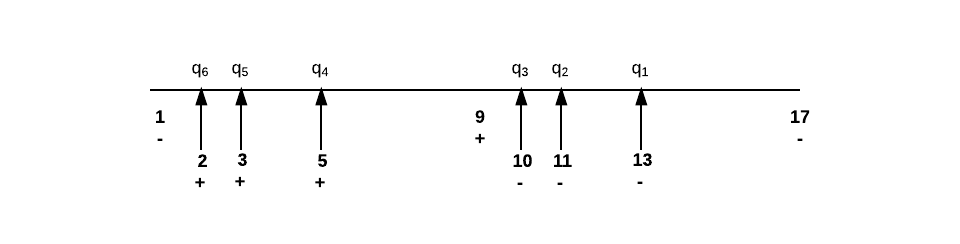
\includegraphics[width=\linewidth]{img/hw1_1d}
  \caption{Query example to decrease version space size.}
\end{figure}
\end{enumerate}

\section{Question 2}
\begin{figure}[H]
  \centering
  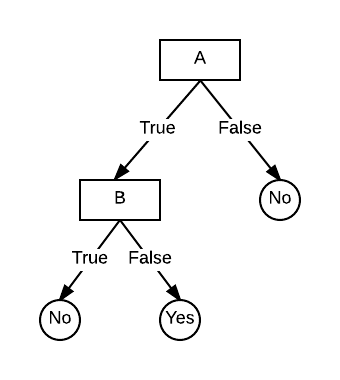
\includegraphics[scale=0.5]{img/hw1_2a}
  \caption{$A \wedge \left[ \thicksim B \right]$}
\end{figure}

\begin{figure}[H]
  \centering
  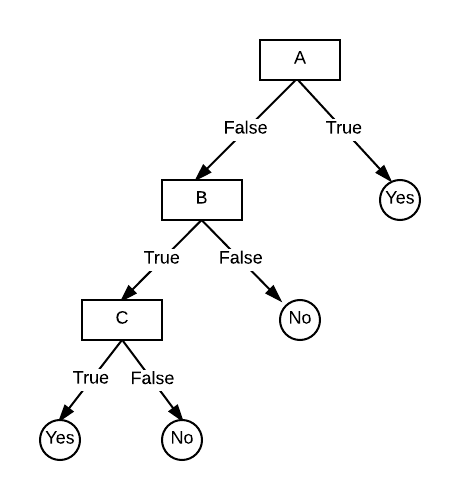
\includegraphics[scale=0.5]{img/hw1_2b}
  \caption{$A\vee\left[ B\wedge C \right]$}
\end{figure}

\begin{figure}[H]
  \centering
  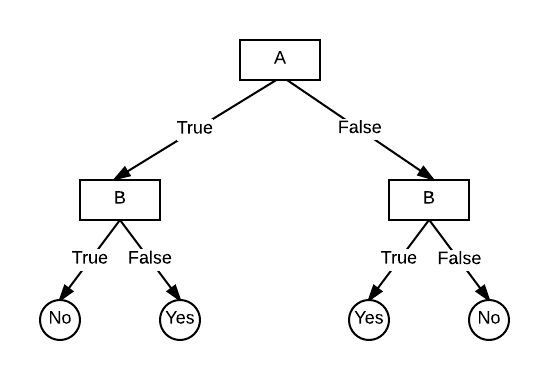
\includegraphics[scale=0.5]{img/hw1_2c}
  \caption{$A\oplus B$}
\end{figure}

\begin{figure}[H]
  \centering
  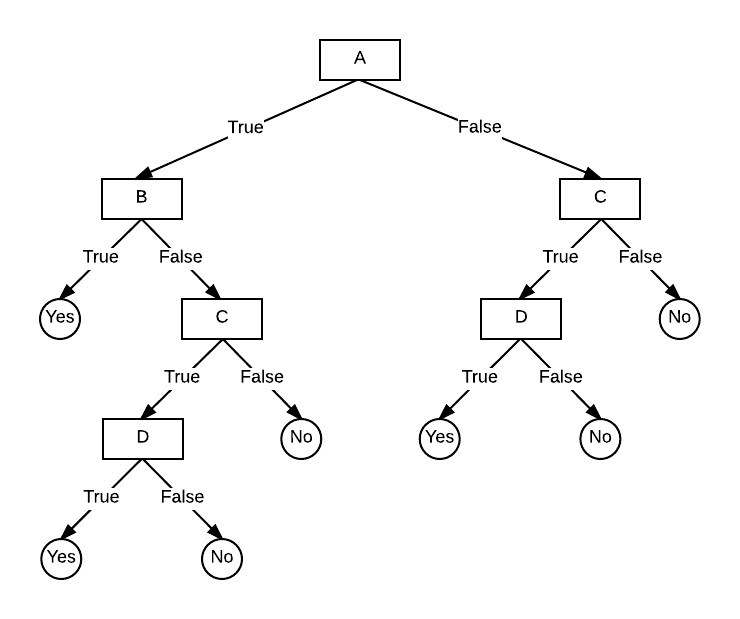
\includegraphics[scale=0.5]{img/hw1_2d}
  \caption{$\left[  A \wedge B\right] \vee \left[  C\wedge D \right]$}
\end{figure}


\section{Question 3}

\begin{enumerate}[(a)]
  \item The entropy of the dataset is calculated as follows:
    \begin{center}
      \begin{align*}
        I&=-{ p }^{ + }\log _{ 2 }{ { p }^{ + } } -{ p }^{ - }\log _{ 2 }{ { p }^{ - } } \\
         &=-\frac { 3 }{ 6 } \log _{ 2 }{ \frac { 3 }{ 6 }  } -\frac { 3 }{ 6 } \log _{ 2 }{ \frac { 3 }{ 6 }  } \\
         &=1
      \end{align*}
    \end{center}
  \item The ID3 algorithm would choose the attribute with smallest impurity which is calculated as below:
    \begin{center}
      \begin{align*}
        { I }^{ \prime  }\left( { a }_{ i } \right) &=\frac { \left| T \right|  }{ \left| T+F \right|  } \left( -{ p }_{ T }^{ + }\log _{ 2 }{ { p }_{ T }^{ + } } -{ p }_{ T }^{ - }\log _{ 2 }{ { p }_{ T }^{ - } }  \right) \\
        &+ \frac { \left| F \right|  }{ \left| T+F \right|  } \left( -{ p }_{ F }^{ + }\log _{ 2 }{ { p }_{ F }^{ + }-{ p }_{ F }^{ - } } \log _{ 2 }{ { p }_{ F }^{ - } }  \right) 
      \end{align*}
    \end{center}
    where $i=1,2$.
    \begin{center}
      \begin{align*}
        { I }^{ \prime  }({ a }_{ 1 })&=\frac { 3 }{ 6 } \left( -\frac { 2 }{ 3 } \log _{ 2 }{ \frac { 2 }{ 3 }  } -\frac { 1 }{ 3 } \log _{ 2 }{ \frac { 1 }{ 3 }  }  \right) +\frac { 3 }{ 6 } \left( -\frac { 1 }{ 3 } \log _{ 2 }{ \frac { 1 }{ 3 } -\frac { 2 }{ 3 } \log _{ 2 }{ \frac { 2 }{ 3 }  }  }  \right) =0.9183 \\
        { I }^{ \prime  }({ a }_{ 2 })&=\frac { 4 }{ 6 } \left( -\frac { 2 }{ 4 } \log _{ 2 }{ \frac { 2 }{ 4 }  } -\frac { 2 }{ 4 } \log _{ 2 }{ \frac { 2 }{ 4 }  }  \right) +\frac { 2 }{ 6 } \left( -\frac { 1 }{ 2 } \log _{ 2 }{ \frac { 1 }{ 2 } -\frac { 1 }{ 2 } \log _{ 2 }{ \frac { 1 }{ 2 }  }  }  \right) =1.0
      \end{align*}
    \end{center}
Since ${ I }^{ \prime  }({ a }_{ 1 })<{ I }^{ \prime  }({ a }_{ 2 })$, \textit{ID3} algorithm would choose $a_1$ next.
\end{enumerate}
\section{Question 4 and 5}

\subsection{Introduction}
We've implemented the ID3 algorithm with impurity as splitting criterion along with rule post-pruning. We used 4 data sets from the UC Irvine Machine Learning Repository. In this report, we present the results of the ID3 algorithm on these data sets.

\subsection{Data}
4 data sets were obtained from UC Irvine Machine Learning
Repository. In addition to the ``Congressional Voting Records
(house-voting-84)'' and ``Monks I'' data sets, we chose ``Nursery''
and ``Tic-Tac-Toe Endgame'' datasets. All of these data sets have
categorical attribute values with number of attributes ranging from 7
to 16. All except the ``Nursery'' data set have binary class labels,
``Nursery'' data set has 5 possible class values. None of the data
sets have missing attribute values except ``Congressional Voting
Records''. Attributes in ``Congressional Voting'' data set take ``?''
as values, however we considered this a legitimate attribute value
carrying information given the context. In addition, we used the
weather data set used in lectures to verify our implementation.  All
data sets can be found in the accompanying archive. Summary of the
data sets can be found in the Table \ref{table:datasetsummary}.

\begin{table}[H]
  \centering
  \begin{small}
    \begin{tabular}{|l|l|l|l|l|}
      \hline
      \textbf{Data Set Name}             & house-votes-84 & monks-1      & tic-tac-toe  & nursery      \\ \hline
      \textbf{Data Set Characteristics}  & Multivariate   & Multivariate & Multivariate & Multivariate \\ \hline
      \textbf{Number of Instances}       & 434            & 556          & 958          & 12960        \\ \hline
      \textbf{Number of Attributes}      & 16             & 7            & 9            & 8            \\ \hline
      \textbf{Attribute Characteristics} & Categorical    & Categorical  & Categorical  & Categorical  \\ \hline
      \textbf{Missing Values?}           & No             & No           & No           & No           \\ \hline
    \end{tabular}
  \end{small}
  \caption{Summary of the selected data sets.}
  \label{table:datasetsummary}
\end{table}

\subsection{Implementation}
We implemented ID3 algorithm with post-pruning with Scala (source code
available in archive). For each data set, we, first, reserved more
than 30 examples sampled randomly without replacement for testing,
then from the remaining training set we extracted at least 30 examples
randomly without replacement for validation. We take these values as
inputs to the ``.properties'' file. After building the tree, we
extracted the rule set by traversing from the root to each leaf. After
obtaining each leaf, we used the validation set to prune these
rules. We dropped a precedent in a rule, if when dropped the modified
rule had better accuracy on the validation set. We sorted the rules
according to their validation accuracy in a decreasing manner.

While predicting the classes of the examples in the test set, we
traversed the tree with each example and whenever an example had an
attribute value unmatched in the tree we used majority voting (see
\ref{discussion}). Prediction with pruned rule set was done by
checking each example against the rules in the rule set beginning with
the rule with highest accuracy. When an example had matching attribute
values with a rule, we used that rule to predict the class, and
continued with the next example.

After running the program the following files can be found:
\begin{itemize}
   \item ``.validation'' contains the examples that were used for pruning the tree.
   \item ``.test'' contains the examples that the tree and the pruned rule set were tested on.
   \item ``.training'' contains the examples left in the training set after test and validation sets are formed.
   \item ``.tree'' contains the tree built by ID3 algorithm, each tab signifies added depth to the tree with a chosen attribute. The attribute used to split the data is indicated by "Decide-on", entropy of the dataset at that node and the impurity of the chosen attribute as well as the number of class members at that node are reported.
   \item ``.prunedRuleSetSorted'' gives the accuracy of each pruned rule on the validation set in sorted order by accuracy
   \item ``.prunedRuleSetUnsorted'' gives the accuracy of each pruned rule on the validation set   
   \item ``.prunedRuleSetTest'' gives the accuracy of each pruned rule on the test set
   \item ``.unprunedRuleSet'' gives the origin rule set extracted from the built tree
   \item ``.unprunedRuleSetTest'' gives the test accuracies of unpruned rules  
\end{itemize}

\subsection{Results}
We observed comparable heights obtained for different datasets. Trees
had heights ranging between 5 and 8 on average over 100 iterations
even though the attribute values change between 7 and 16. However, the
number of nodes ranged between 21 and 320 on average over 100
iterations (Table \ref{table:datasetsummary}, Table \ref{table:performance}).

\begin{table}[H]
  \centering
  \begin{small}
    \begin{tabular}{|l|l|l|l|l|}
      \hline
      \textbf{Data Set Name}                           & house-votes-84 & monks-1 & tic-tac-toe & nursery \\ \hline
      \textbf{Avg. number of nodes}                           & 21.01                   & 38.95            & 112.51               & 319.79           \\ \hline
      \textbf{Avg. height}                                & 7.23                    & 5.21             & 7.33                 & 8.0                \\ \hline
      \textbf{Avg. accuracy of tree on test data}         & 0.936                   & 0.966            & 0.833                & 0.983            \\ \hline
      \textbf{Avg. accuracy of pruned rules on test data} & 0.943                   & 0.984            & 0.861                & 0.996            \\ \hline
    \end{tabular}
\end{small}
\caption{Results of 100 iterations (Validation size = 30, Test size = 30).}
\label{table:performance}
\end{table}

We always observed higher accuracies for the pruned rule set than the
tree. This means that overfitting took place while building the tree,
i.e we can find an alternative hypothesis with higher training but
lower test error. Pruning the rules improved accuracy (Figures
\ref{fig:house-comp}, Figure \ref{fig:monk-comp}, and Figure
\ref{fig:tictactoe-comp}).

\begin{figure}[H]
  \centering
  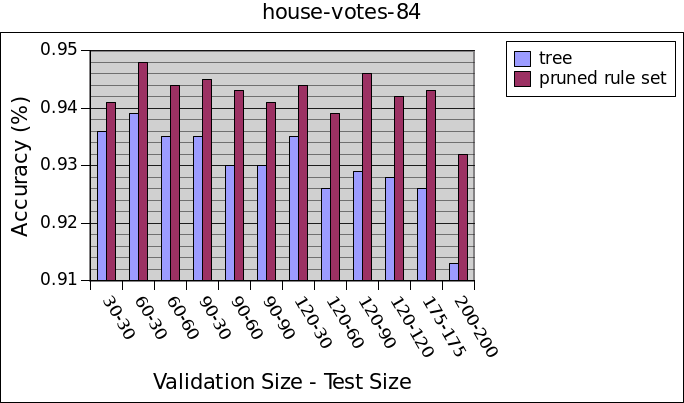
\includegraphics[scale=0.5]{img/house-votes-84-comparison}
  \caption{Accuracy comparison of tree and post pruning on house-votes-84 test data with changing training data size.}
  \label{fig:house-comp}
\end{figure}

\begin{figure}[H]
  \centering
  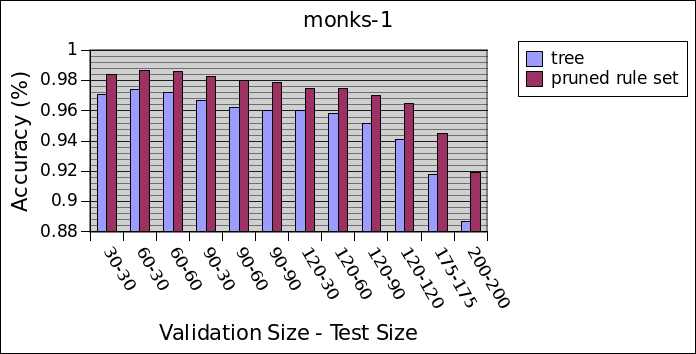
\includegraphics[scale=0.5]{img/monks-1-comparison}
  \caption{Accuracy comparison of tree and post pruning on monks-1 test data with changing training data size.}
  \label{fig:monk-comp}
\end{figure}

\begin{figure}[H]
  \centering
  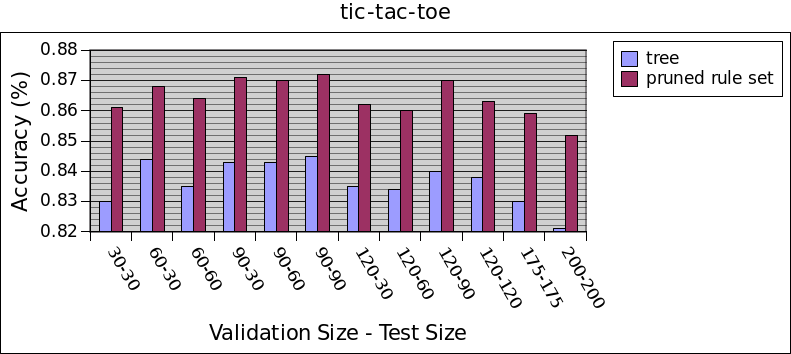
\includegraphics[scale=0.5]{img/tic-tac-toe-comparison}
  \caption{Accuracy comparison of tree and post pruning on tic-tac-toe test data with changing training data size.}
  \label{fig:tictactoe-comp}
\end{figure}



\subsection{Discussion}\label{discussion}
We observed comparable tree heights and different node numbers for
different datasets. All trees except for ``Congressional Voting'' have
heights that are about the same as their attribute numbers. This would
mean for the ``Congressional Voting'' data set, that 7 attributes are
enough to classify an example despite the larger available attribute
number. The number of nodes in ``Tic-Tac-Toe'' and ``Nursery'' data sets
were much larger than in ``Monks-I'' and ``Congressional Votes'' data sets,
this is commensurate with the number of available values for
attributes in each data set (Table \ref{table:datasetsummary}, Table \ref{table:performance}).

During implementation, we were faced with a number of issues. First,
during prediction of novel examples using the tree, some of the
attributes had values in test data that were not present in our
tree. For example, while our tree could split the data into ``hot''
and ``cool'' values of temperature attribute, it couldn't decide which
subset an example with ``mild'' temperature value belonged to
(depicted as in Figure \ref{fig:majority-vote}) . In that case, we
opted for sending the example as deep in the tree as possible, then
classifying the example as a member of the group with highest
frequency in that node. If there were more than one classes with the
highest frequency we picked the class randomly.

\begin{figure}[H]
  \centering
  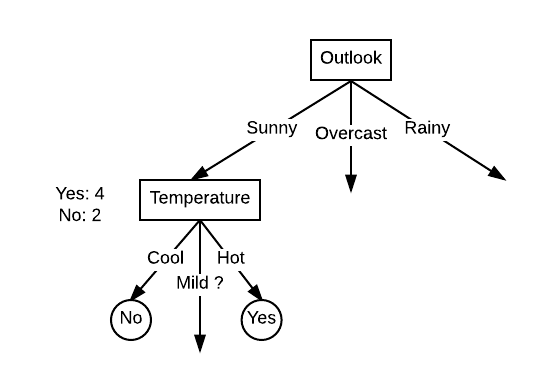
\includegraphics[scale=0.5]{img/majority_voting}
  \caption{Depiction of classifying the example as a member of the group with the highest frequency.}
  \label{fig:majority-vote}
\end{figure}

During pruning, there was another issue we had to make a
implementation decision upon. After building the tree and obtaining
the rules, some of the rules applied to none of the examples in the
validation set. Similarly, we observed the same issue even with rules
with reduced precedents. In those cases, we dropped a precedent only
if the modified rule (rule with the precedent dropped) applied to an
example and it's accuracy was at least $0.9$. In other cases, where the
rule (with the precedent we were considering dropping) applied to some
examples, we only dropped the precedent if the modified rule had
higher accuracy than the unmodified rule.

To gauge overfitting, we decreased the size of the training set. We
observed a steady decrease in the average accuracy of both the tree
and the pruned rule set in ``Monks-1'' data, although the decrease was
more obvious in the tree predictions as depicted in Figure
\ref{fig:monk-comp}. This could mean that overfitting occurs when the
data is not sufficiently large because the algorithm is not presented
with enough examples to detect true rules. However, this was not the
case for other datasets with comparable sizes.

\end{document}